\graphicspath{{./figs/Chp-Bg/}}

\chapter{Background}
\label{chp:bg}


\section{Sparse Linear Systems}

Using methods such as the \gls{acr:fem} and the \gls{acr:fdm} to solve linear \glspl{acr:pde} commonly results in a sparse linear system of equations taking the algebraic form:
\begin{equation}
	Au=b \label{eqn:aub}
\end{equation}
where $A$ is a sparse square matrix of order $N$; $u$ is a vector of unknowns; and $b$ is the right-hand side (or source) vector.
The term ``sparse'' refers to the fact that the matrix $A$ is made up of mostly zero off-diagonal elements.
The size of the discretized \gls{acr:pde} problem is characterized by $N$, or by the number of non-zeros (\gls{acr:nnz}) which is also proportional to $N$ such that $\bigo{\gls{acr:nnz}} = \bigo{lN}$, where $l$ is a constant factor.
An important feature of sparse problems is that the factor $l$ is independent of $N$.
In addition, $l$ is also considerably smaller than $N$ ($l \ll N$).
For example, $l$ can be found to be in the range between five to a few hundreds, in some rare cases, while $N$ can scale indefinitely to millions or more depending on the desired discretization level of the \gls{acr:pde} domain.
This feature is mainly due to the discretization process, or meshing, which results in fixed local connectivities for each node irrespective of the size of the mesh.
This can clearly be illustrated by considering a regular rectangular grid.
Any interior node will always be surrounded by four rectangles even if the domain size is enlarged or the mesh density is increased by increasing the number of elements.
Since off-diagonal elements in the matrix $A$ indirectly represent coupling between nodes, uncoupled elements in the mesh will result in uncoupled nodes and consequently zero off-diagonals in $A$.
This concept also applies to irregular meshes of arbitrary element geometries, however the local connectivity would slightly vary from one node to another.

Sparse solvers can exploit the sparsity of the problem in order to gain considerable memory and computational advantages.
For example, if we would solve the linear system \eqnRef{eqn:aub} by directly taking the inverse of $A$ using a dense solver, the solver would require $\bigo{N^2}$ memory and $\bigo{N^3}$ computational operations.
In contrast, sparse solvers in general would require $\bigo{N}$ memory and $\bigo{N^d}$ computational operations where $d$ typically is $d \in [1, 3]$.
However, we will later see that certain iterative solvers such as multigrid schemes achieve optimal convergence scalability with $d=1$ for elliptic \glspl{acr:pde}.

Nonetheless, implementing sparse linear systems on \gls{acr:hpc} platforms is difficult.
This is mainly due to the fact that sparse systems resulting from complex geometries can exhibit irregular sparsity patterns which can negatively impact their computational efficiency.
To illustrate this issue, we present a brief overview of sparse data-structures and solvers.


\subsection{Sparse Data-Structures}

Discretization of simple domains using the \gls{acr:fdm} can mostly result in sparse systems that exhibit regular sparsity patterns.
The sparse matrices for such systems typically have banded structures, where the non-zeros are extended along the diagonal of the matrix.
Standard techniques to handle these systems are widely available and usually result in very efficient \gls{acr:hpc} execution.
However, the \gls{acr:fdm} method lacks the general applicability offered by the \gls{acr:fem} method which enjoys a much wider use in the engineering and scientific community \cite[p. 19]{bib:Jin2002TFEMIE}.
The \gls{acr:fem} method, on the other hand, exhibits a more degraded \gls{acr:hpc} performance if specialized techniques are not used.
This degraded performance is mainly due to the irregular sparsity pattern of the matrix $A$.
\figRef{fig:sparseMat} shows sample sparse \gls{acr:fem} matrices clearly illustrating its irregular sparsity patterns.
Solutions for such systems will be the primary focus of our work.

\begin{figure}
	\centering
	\subfloat[]{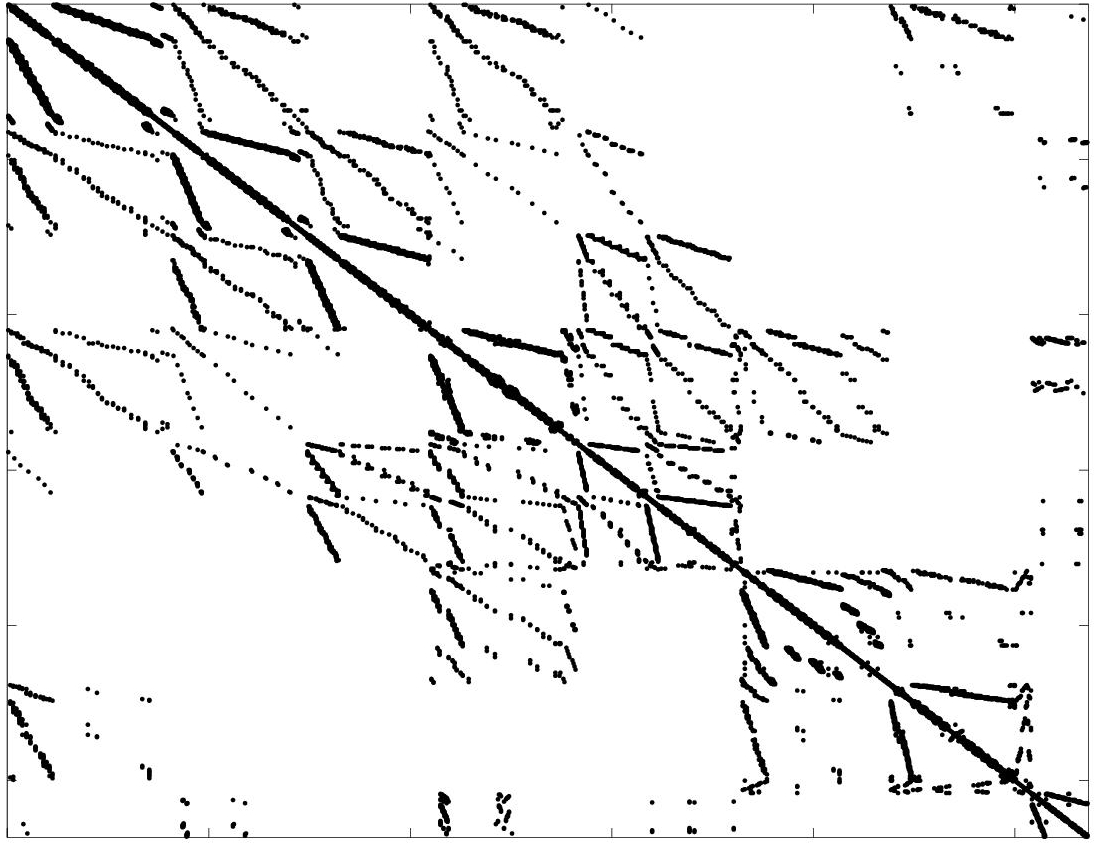
\includegraphics[scale=.23]{can_1072_1072_12444.jpg} \label{fig:sp_1}}
  %\hspace{+1mm}
	\subfloat[]{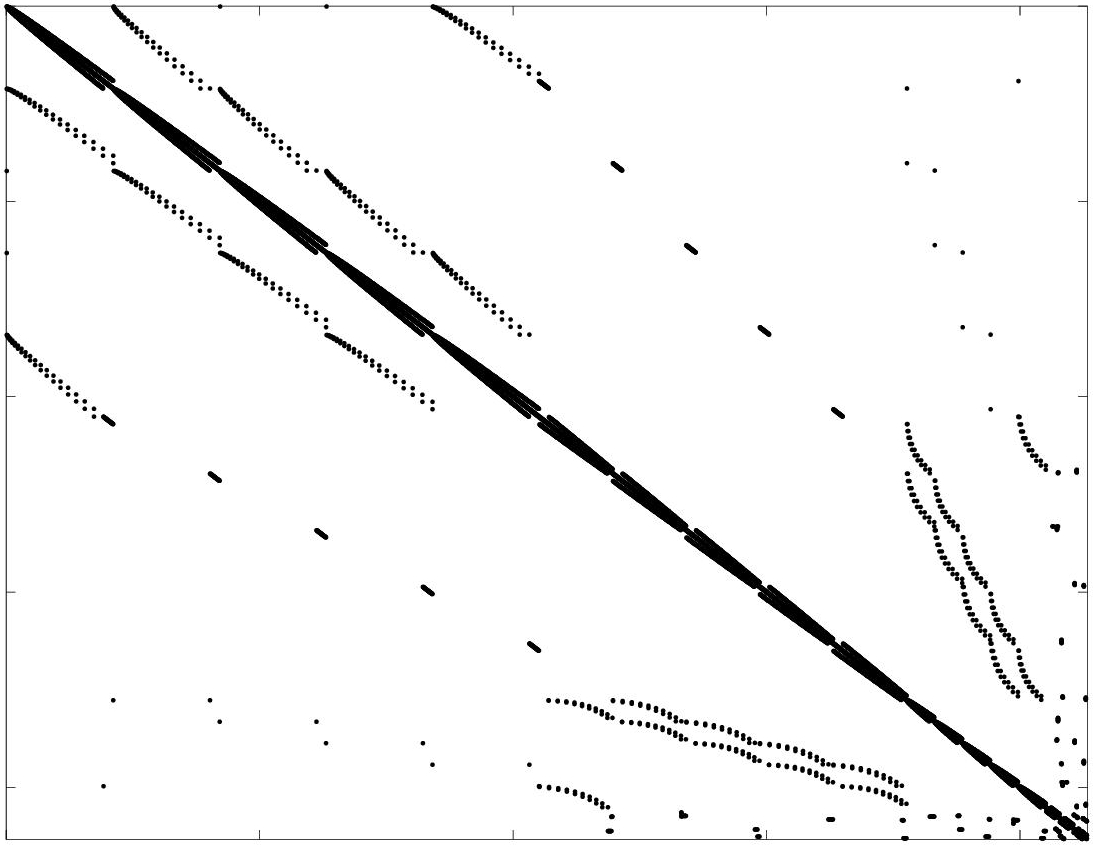
\includegraphics[scale=.23]{blackhole_2132_14872.jpg} \label{fig:sp_2}
	}
  %\hspace{-1mm}
	\subfloat[]{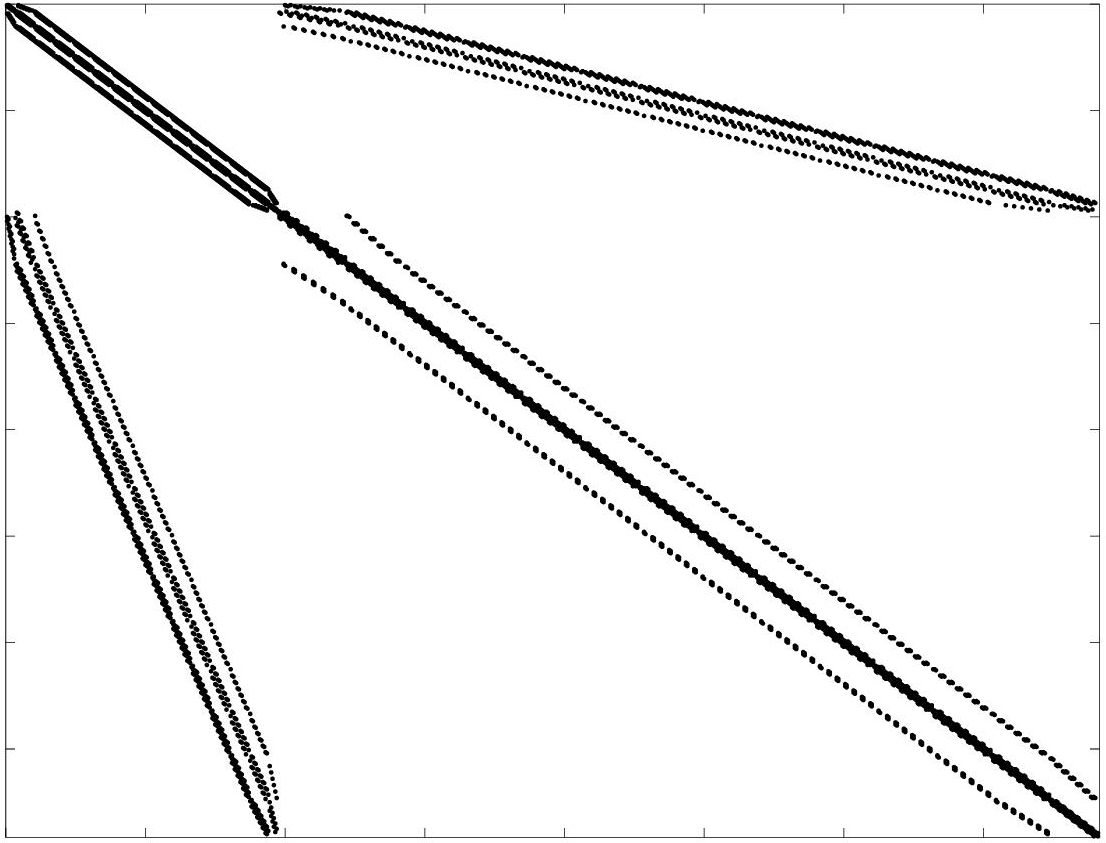
\includegraphics[scale=.23]{bfw782b_782_5982.jpg} \label{fig:sp_3}
	}
	\caption[Samples of sparse matrices.]{Samples of sparse matrices resulting from different \gls{acr:fem} application areas. The matrices are obtained from the Matrix Market online repository \cite{bib:matrixMarket} and plotted using Octave \cite{bib:octave2012}. The application areas are: \protect\subref*{fig:sp_1} Aircraft structure, matrix name: ``can 1027'' $N=1027$ $\gls{acr:nnz}=12444$. \protect\subref*{fig:sp_2} Structural engineering, matrix name: ``blackhole'' $N=2132$ $\gls{acr:nnz}=14872$.  \protect\subref*{fig:sp_3} Waveguide, matrix name: ``bfw782b'' $N=782$ $\gls{acr:nnz}=5982$.}
	\label{fig:sparseMat}
\end{figure}

Sparse data-structures mainly store the non-zero elements of the matrix and their locations based on their row and column indices.
However, the arrangement of the data-structure will need to support two key objectives.
The first objective is to minimize the overall data-structure size by reducing the overhead data, such as pointers, indices, and zero paddings if needed.
The second objective is to organize the data-structure in such a way to hide the memory access latencies and improve the memory bandwidth utilization for basic sparse operations such as the \gls{acr:smvm}.
Obtaining good performance for sparse solvers on \gls{acr:hpc} platforms usually requires balancing the trade-offs from these two objectives.
At the present time however, memory chips can be provided at commodity prices while memory bandwidth (connectivity with the CPU) remains limited; as a result, the second objective will usually have more impact on performance than the first one.

Examples of commonly used sparse data-structure formats are the \gls{acr:cc}, the \gls{acr:csr}, the \gls{acr:csc}, and the \gls{acr:jd}.
In the \gls{acr:cc} format, each non-zero is stored along with its row and column indices; hence, the \gls{acr:cc} format is known to be the simplest and most flexible of all formats.
The \gls{acr:cc} format however requires the largest overhead to store.
The \gls{acr:csr} format, on the other hand, requires less memory and performs relatively better for sparse operations such as the \gls{acr:smvm}, hence it became one of the most popular formats.
\figRef{fig:sparseFormats} illustrates a simple example of the \gls{acr:cc} and the \gls{acr:csr} formats.

\begin{figure}[h]
	\centering
	\subfloat[]{%
	\begin{minipage}[c]{0.5\textwidth}%
		\[
		A=\left[\begin{array}{ccccc}
			1. & 0. & 6. & 0. & 0.\\
			0. & 2. & 0. & 0. & 0.\\
			6. & 0. & 3. & 0. & 0.\\
			0. & 0. & 0. & 4. & 8.\\
			0. & 0. & 0. & 8. & 5.
		\end{array}\right]
		\]
	\end{minipage}%
	\label{fig:ssp}}
	\vfill
	\subfloat[]{%
	\begin{minipage}[c]{\textwidth}%
		\centering
		\begin{tabular}{l|lllllllll|}
			\cline{2-10} 
			$Ae$         & 1. & 2. & 3. & 4. & 5. & 6. & 6. & 8. & 8.\tabularnewline
			\cline{2-10}
			\multicolumn{10}{l}{}\\[-2ex]
			\cline{2-10}
			$Ri$         & 1  & 2  & 3  & 4  & 5  & 1  & 3  & 4  & 5\tabularnewline
			\cline{2-10}
			\multicolumn{10}{l}{}\\[-2ex]
			\cline{2-10}
			$Ci$         & 1  & 2  & 3  & 4  & 5  & 3  & 1  & 5  & 4\tabularnewline
			\cline{2-10} 
		\end{tabular}
	\end{minipage}
	\label{fig:cc}
	}
	\vfill
	\subfloat[]{%
	\begin{minipage}[c]{\textwidth}%
		\centering
		\begin{tabular}{l|lllllllll|}
			\cline{2-10} 
			$Ae$         & 1. & 6. & 2. & 6. & 3. & 4.                      & 8. & 8. & 5.\tabularnewline
			\cline{2-10}
			\multicolumn{10}{l}{}\\[-2ex]
			\cline{2-10}
			$Ri$         & 1  & 3  & 2  & 1  & 3  & 4                       & 5  & 4  & 5\tabularnewline
			\cline{2-10}
			\multicolumn{10}{l}{}\\[-2ex]
			\cline{2-7}
			$Rp$         & 1  & 3  & 4  & 6  & 8  & \multicolumn{1}{l|}{10} &    &    & \multicolumn{1}{l}{}\tabularnewline
			\cline{2-7} 
		\end{tabular}
	\end{minipage}
	\label{fig:csr}
	}
	\caption[Examples of two sparse data-structure formats.]{Examples of two sparse data-structure formats where $Ae$ is the elements list of the matrix $A$, $Ri$ is the element row index list, $Ci$ is the element column index list, and $Rp$ is the row start index list. \protect\subref*{fig:ssp}~The sparse matrix. \protect\subref*{fig:cc}~The \gls{acr:cc} format. \protect\subref*{fig:csr}~The \gls{acr:csr} format.}
	\label{fig:sparseFormats}
\end{figure}


\subsection{Sparse Linear Solvers}

Sparse linear solvers mainly fall into two categories, sparse direct solvers and sparse iterative solvers.
Sparse direct solvers perform some type of LU or Cholesky factorization while reducing the effect of fill-ins.
Fill-in is a side-effect of direct sparse solvers that occurs from the factorization process by introducing non-zeros in locations that were zeros in the original sparse matrix.
The effect of fill-in can negatively impact the CPU's performance by progressively increasing the memory and the computational requirements.
Widely used open-source libraries for sparse direct solvers include UMFPACK \cite{bib:UMFPACKDavis2004,bib:Davis2004CPS}, SuperLU \cite{bib:SuperLU,bib:SuperLUUG}, and MUMPS \cite{bib:MUMPS}.
Specialized matrix reordering algorithms such as the \gls{acr:md} \cite{bib:George1989TEOTMDOA} reordering and the \gls{acr:nd} \cite{bib:George1973NestedDisssection} reordering can help in reducing the amount of fill-ins.
Sparse direct solvers can be particularly efficient for problems requiring multiple solutions for different right hand side vectors (different $b$ vectors in \eqnRef{eqn:aub}), since only forward-backward substitution is needed to be applied on each right hand side after the first solve.
Due to fill-in that substantially increases in 3D problems, the performance of sparse direct solvers is particularly worse than iterative solvers.
A sparse Cholesky factorization would require $\bigo{N^2}$ operations and $\bigo{N^{4/3}}$ memory for discretized 3D Poisson's problems \cite[p.~278]{bib:Demmel1997anla}.
Therefore, iterative solvers are more popular in \gls{acr:hpc} applications because they scale more efficiently for larger problems in terms of both memory requirement and execution time.
In fact, certain iterative solvers can achieve the optimal computational time of $\bigo{N}$ and the optimal memory space of $\bigo{N}$ such as multigrid solvers or preconditioners.
Henceforth, our focus in this work will be directed towards iterative solvers.
In particular, we consider applications that result in linear systems with $A$ being \gls{acr:spd}.
Such a property is commonly present in linear systems generated by a wide range of \gls{acr:fem} applications.
Also, certain methods developed for \gls{acr:spd} matrices can be generalize to non-symmetric positive definite matrices such as the \gls{acr:bicg} method or, for more general definite systems, the \gls{acr:gmres} method.
However, the two methods, the \gls{acr:bicg} and the \gls{acr:gmres}, are considered specializations of a wider class of solvers known as the \acrfullpl{acr:ksm}.


Two widely used iterative solvers are the \gls{acr:cg} method and the multigrid scheme.
Extensive literature is devoted to these methods since their early conception.
Recent references that introduce the theory, as well as various implementation approaches, include \cite{bib:Saad2003IMFSLS2E,bib:Demmel1997anla,bib:Demmel1994Templates,bib:Golub1996MC,bib:Briggs2000AMT,bib:Trottenberg2001M,bib:Shewchuk1994ICG}.
The \gls{acr:cg} method in particular, which was first introduced in 1950, only found wide use in the early 1970s when the efficiency of the method was vastly improved by the introduction of preconditioning \cite{bib:Golub1989SHC}.  
In the following sections we provide a brief overview of these methods.


\subsection{The Preconditioned Conjugate Gradient}
\label{sec:pcg}

The \gls{acr:cg} algorithm, applicable when $A$ is \gls{acr:spd}, is a special case of a more general class of algorithms referred to as \glspl{acr:ksm}.
In such algorithms, the sequence of approximate solutions $u_m$ are taken from an evolving subspace spanned by vectors resulting from repeatedly applying the matrix $A$ on the initial residual $r_0 = b-Au_0$.
Such a space is referred to as the Krylov-subspace and is denoted as $\mathcal{K}_m = \OpN{span}\{r_0,Ar_0,A^2r_0,\cdots,A^{m-1}r_0\}$.
The \gls{acr:cg} algorithm can be viewed as a search direction algorithm that obtains $A$-orthogonal (conjugate) directions from the search space $\mathcal{K}_m$ in order to minimize the following quadratic:
\begin{equation}
	\mathcal{Q}(u) = \frac{1}{2}u^TAu-b^Tu + c \label{eqn:quad}
\end{equation}
where $c$ is a constant.
It can be shown that the optimum point, ($u_\star$), satisfies the gradient of $\mathcal{Q}$ such that $\nabla\mathcal{Q}\mid_{u=u_\star} = Au_\star - b = 0$.
Using the residuals as the conjugating vectors in the Gram-Schmidt orthogonalization process results in the elaborate \gls{acr:cg} algorithm.
A key advantage of using conjugated directions is that in each iteration the error is not only being minimized in the current search space, but rather in all subspaces of the search space.
As a result, the \gls{acr:cg} algorithm theoretically reaches the optimal solution in $N$ iterations.
In practice however, the \gls{acr:cg} algorithm converges in less than $N$ iterations; for example, in Poisson's problems the convergence is upper-bounded by $\bigo{N^{3/2}}$ for 2D and $\bigo{N^{4/3}}$ for 3D \cite{bib:Shewchuk1994ICG}.
Preconditioning considerably improves the convergence of \gls{acr:cg} by improving the characteristics of the matrix $A$ at the expense of an additional computational cost per each iteration.
In \gls{acr:pcg}, a \gls{acr:spd} preconditioner matrix ($M$) is selected to approximate $A$ such that the residuals can be made $M^{-1}$-orthogonal.
Clearly for the preconditioning process to be efficient, $M$ must be considerably easier to solve than $A$.
The \gls{acr:pcg} algorithm pseudocode is listed in \algRef{alg:pcg}.  
The key computational kernels in the \gls{acr:pcg} algorithm are the \gls{acr:smvm}, shown in Line~\ref{alg:smvmLine}, and the preconditioner solve step, shown in Line~\ref{alg:precLine}.

\begin{algorithm}
  %\centering
	\begin{algorithmic}[1]
		\STATE \textbf{initialize:}
		\STATE ~ ~$r_0 = b - Au_0$
		\STATE ~ ~\text{solve: } $M z_0  = r_0$
		\STATE ~ ~$d_0 = z_0$
		\REPEAT[Iterate $t=1,2,\cdots$]
		\STATE $\theta_t = z_t^Tr_t$
		\STATE $v_t = Ad_t$ \label{alg:smvmLine}
		\STATE $\rho_t = \frac{\theta}{d_t^Tv_t}$
		\STATE $u_{t+1} = u_t + \rho_t d_t$
		\STATE $r_{t+1} = r_t - \rho_t v_t$
		\STATE \text{solve: } $z_{t+1} M = r_{t+1}$ \label{alg:precLine}
		\STATE $\theta_{t+1} = z_{t+1}^Tr_{t+1}$
		\STATE $ \gamma_t = \frac{\theta_{t+1}}{\theta_t}$
		\STATE $d_{t+1} = z_{t+1} + \gamma_t d_t $
		\UNTIL{convergence: $r_{t+1}$ sufficiently small}
		\STATE \textit{Output:} $u_{t+1}$
	\end{algorithmic}
	\caption[The \acrshort{acr:pcg} algorithm.]{The \glsfirst{acr:pcg} algorithm.}
	\label{alg:pcg}
\end{algorithm}



\subsection{The Multigrid Scheme}
\label{sec:RMG}

Multigrid accelerated solvers \cite{bib:Briggs2000AMT,bib:Trottenberg2001M,bib:multigridZhu2006} are among the fastest known algorithms to obtain solutions to linear systems of equations resulting from the \gls{acr:fem}.
The performance of multigrid can, in practice, be shown to be independent of the size of the finest discretization of the domain \cite{bib:Briggs2000AMT,bib:Trottenberg2001M}, attaining the optimal complexity of $\bigo{N}$ for both computation and memory.
In this section we present the general principles behind the multigrid scheme.


Multigrid schemes are based on creating different levels of approximations to a problem so as to obtain progressively lower complexities, or lower number of unknowns, on each sub-level.
An approximate solution can be obtained very quickly on the lowest complexity level.
The approximate solution is then transferred progressively to the problem's actual level of accuracy.
This process is repeated iteratively in the hopes of speeding-up the overall computation time.
The problem levels have to be related according to a criterion, otherwise the approximated solution can not be relayed across the adjacent levels.
In the case of \gls{acr:fem} applications, different problem levels can be created by performing nested mesh refinement, referred to as hierarchical mesh refinement.
Such hierarchical meshing schemes are obtained by splitting each mesh element into smaller elements.
Multigrid schemes using hierarchical meshes are referred to as the \gls{acr:gmg}.
An example of an \gls{acr:fem} library that uses \gls{acr:gmg} is the open-source library \dealName{} \cite{bib:dealii2007}.
Alternatively, different levels of problem operators can be generated using algebraic operations on the matrix $A$, such multigrid schemes are referred to as the \gls{acr:amg}.


The key advantage of \gls{acr:amg} schemes is that they are designed to be used as black-box solvers where all that is needed from the underlying \gls{acr:pde} problem is the sparse linear system \eqnRef{eqn:aub}.
An example of a solver library that uses \gls{acr:amg} is the open-source library BoomerAMG~\cite{bib:boomerAMG}.
\Gls{acr:amg} solvers are used in frameworks where the sparse matrix $A$ is assembled once on the finest level.
However, an \gls{acr:amg} solver requires a number of global sparse algebraic operations as well as processing a number of sparse data-structures for each generated level operator.
While \gls{acr:gmg}, on the other hand, provides the potential of implementing matrix free operations.
In addition, \gls{acr:gmg} performs considerably better because it can better utilize the inherent problem structure in the hierarchical \gls{acr:fem} mesh to lower the computational complexity.
Therefore, it is advisable to use \gls{acr:amg} only when it is impossible, or difficult, to setup \gls{acr:gmg}.
Hence, the choice weather to use \gls{acr:amg} or \gls{acr:gmg} is more application dependent than it is performance dependent.
Our work, described in \chpRef{chp:FMGaBP}, utilizes \gls{acr:gmg} schemes to accelerate a parallel formulation of the \gls{acr:fem} problem.


To illustrate the key formulations behind the multigrid solvers, we provide here a brief overview of the two-grid correction scheme.
Given an initial discretization for a continuous bounded domain $\Omega$, refereed to as a coarse mesh $\Omega^H$, then the mesh is refined further by element splitting schemes into a finer mesh $\Omega^h$.
This refinement scheme is illustrated in \figRef{fig:LSM}.
The multigrid correction scheme is based on the simple reformulation of the linear system $Au=b$ into the residual-correction scheme.
Given an exact solution $u_\star$ and an initial approximation $\tilde{u}$, then the correction $z$ can be stated as:
\begin{equation}
	z = u_\star - \tilde{u}. \label{eqn:crr}
\end{equation}
We start by finding the residual:
\begin{equation}
	r = b - A\tilde{u}, \label{eqn:res}
\end{equation}
then the solution to the system $Au=b$ can alternatively be obtained by solving for the correction as:
\begin{equation}
	Az=r, \label{eqn:azr}
\end{equation}
with the initial guess $z=0$. 
The obtained correction $z$ is then added to the initial approximation $\tilde{u}$ to obtain the solution as:
\begin{equation}
	u_\star = z + \tilde{u}.
\end{equation}

The residual-correction reformulation has no computational advantage in itself; however, this reformulation is converted into an iterative process by multigrid.
Using multigrid, the correction in \eqnRef{eqn:azr} is rather computed on a coarse grid (smaller version of $A$) which is then used to compute an improved initial approximation for the fine grid.
We expect an overall computational advantage, since working on the coarse grid is cheaper than working on the fine grid.

\begin{figure}
	\centering
	\subfloat[]{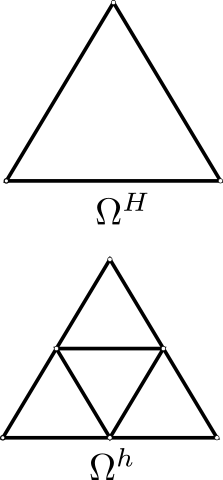
\includegraphics[scale=.3]{tri_split} \label{fig:split}}
  %\hspace{+1mm}
	\subfloat[]{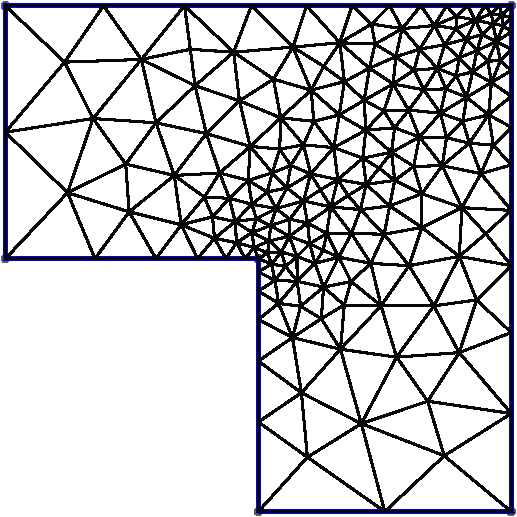
\includegraphics[scale=.5]{LSC} \label{fig:LSC}
	}
  %\hspace{-1mm}
	\subfloat[]{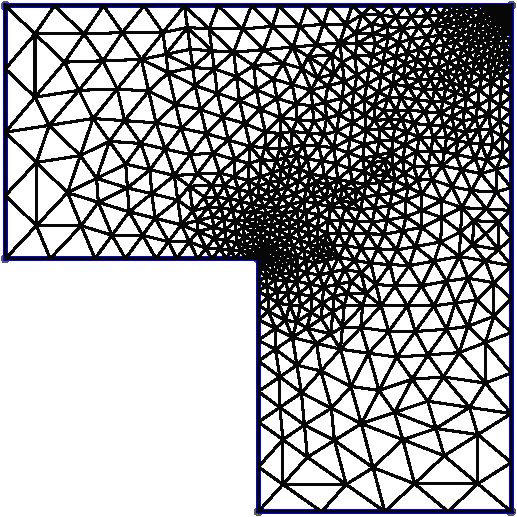
\includegraphics[scale=.5]{LSF} \label{fig:LSF}
	}
	\caption[Mesh refinement by splitting.]{\protect\subref*{fig:split} Mesh refinement by splitting each triangle in mesh $\Omega^H$ into four geometrically similar sub-triangles to produce a finer mesh $\Omega^h$. \protect\subref*{fig:LSC} Sample coarse irregular mesh.  \protect\subref*{fig:LSF} The refined mesh by splitting.}
	\label{fig:LSM}
\end{figure}

We redefine the linear system in \eqnRef{eqn:aub} as $A^h u^h = b^h$; where the superscript $h$ represents the linear system of the fine mesh $\Omega^h$. 
If the superscript $H$ is used, then the system represents the coarse mesh.
The listing in \algRef{alg:2VMG} shows the detailed operations of the two-grid V-cycle multigrid.
A single iteration of the algorithm is refereed to as a V-cycle which reflects the behavior of the algorithm in transferring approximations from fine to coarse grids and then back from coarse to fine grids.
Other key components of the algorithm are the restriction and prolongation operators.
The restriction operator $\mathcal{R}_{h}^{H}$ acts on the residual from the fine grid by mapping it from the fine grid onto the coarse grid using restriction.
On the other hand, the prolongation operator $\mathcal{I}_{H}^h$ acts on the correction from the coarse grid by mapping it onto the fine grid using interpolation.
Since restriction and prolongation operators act on the global residual and correction vectors, they are in fact some form of global sparse operations.
However, in certain applications, such as the \gls{acr:fdm}, these operators can be performed on a point-by-point basis.
In linear transfer operations, the dimensions of $\mathcal{R}$ is given by $(N_H\times N_h)$ where $N_H$ is the number of unknowns in the coarse grid, while $N_h$ is the number of unknowns in the fine grid.
On the other hand, the dimension of $\mathcal{I}$ is $(N_h\times N_H)$.
This residual-correction scheme is also effective in progressively minimizing the error added due to both the restriction and the prolongation operations as the approximate solution on the fine grid approaches the exact solution.
In addition, since the problem has a unique solution, it can be shown that the whole multigrid process can be viewed as a fixed-point process for the exact solution on the fine grid.

\begin{algorithm}[t]
  %\centering
  %\begin{framed}
	\begin{algorithmic}[1]
		\STATE Set initial guess $z^{h}_0=0$
		\REPEAT[V-cycle iterate]
		\STATE Obtain the approximate solution $\tilde{u}^{h}_0$ from $A^h u^h = b^h$ on the fine grid $\Omega^h$ using $v_1$ iterates (pre-smoothing) of a relaxation algorithm with initial guess $z^{h}_0$.\label{alg:fg}
		\STATE Compute the residual $r^h = b^h - A^h \tilde{u}^{h}_0$.
		\STATE Restrict the residual on the coarse grid $\Omega^H$ using $r^H = \mathcal{R}_{h}^{H} r^h$, where $\mathcal{R}_{h}^{H}$ is a fine-to-coarse restriction operator.
		\STATE Obtain the coarse grid correction $\tilde{e}^H$ by solving $A^H e^H = r^H$ with initial guess $e^H = 0$.\label{alg:crr}
		\STATE Compute $z^{h}_1 = \tilde{u}^{h}_0 + \mathcal{I}_{H}^h \tilde{e}^H$, where $\mathcal{I}_{H}^h$ is a coarse-to-fine prolongation operator.
		\STATE Obtain the approximate solution $\tilde{u}^{h}_1$ from $A^h u^h = b^h$ using $v_2$ iterates (post-smoothing) with initial guess $z^{h}_1$.
		\STATE Set new initial guess $z^{h}_0 = \tilde{u}^{h}_1$.
		\UNTIL{Convergence on fine grid.}
	\end{algorithmic}
  %\end{framed}
	\caption{The two-grid V-cycle multigrid process.}
	\label{alg:2VMG}
\end{algorithm}

To elaborate more on the behavior of the restriction and the prolongation operations, we consider a simple example using a 2D quadrilateral mesh shown in \figRef{fig:grid_trans_a}
The coarse mesh contains only one quadrilateral element, while the fine mesh contains four refined quadrilateral elements by splitting the coarse grid element evenly.
The nodal numbers on the diagram reflect global numbering of the indices.
Similarly as indicated in \figRef{fig:grid_trans_b}, a triangular mesh can be refined by splitting a triangular element into four geometrically similar child triangles.
This splitting is performed by connecting nodes inserted at the mid point of each edge in the parent triangle.
\begin{figure}[t]
	\centering
	\subfloat[]{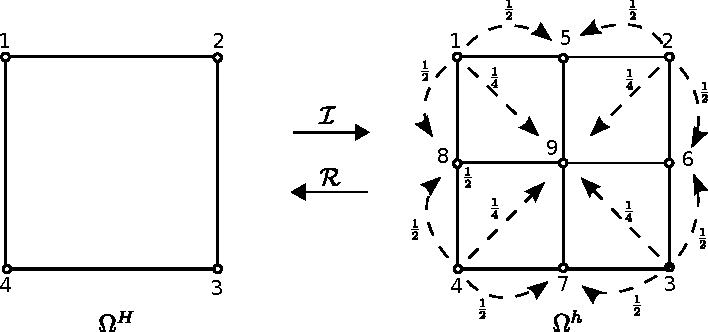
\includegraphics[scale=.8]{grid_trans_a} \label{fig:grid_trans_a}}
	\vfill
	\subfloat[]{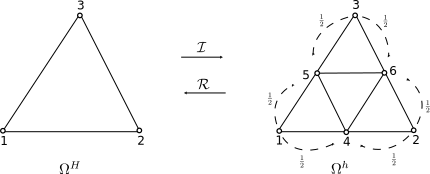
\includegraphics[scale=.8]{grid_trans_b} \label{fig:grid_trans_b}}
	\caption[Multigrid transfer operations.]{Grid transfer operations between: \protect\subref*{fig:grid_trans_a} two 2D quadrilateral meshes and  \protect\subref*{fig:grid_trans_b} 2D triangular meshes. The fractions indicated on the fine meshes represent nodal weightings for the case of linear interpolation.}
	\label{fig:grid_trans}
\end{figure}


The prolongation operator $\mathcal{I}_H^h$ can be defined using linear interpolation.
In linear interpolation, the correction values of the fine grid nodes, which do not overlap the coarse grid nodes, are obtained by averaging the surrounding nodes from the coarse grid.
The overlapping nodes on the fine grid can retain the same correction values from the coarse grid.
Hence the operator $\mathcal{I}_H^h$ matrix can be defined as:
\begin{equation}
	\mathcal{I}_{H}^{h}=\left[\begin{array}{cccc}
		1 & 0 & 0 & 0\\
		0 & 1 & 0 & 0\\
		0 & 0 & 1 & 0\\
		0 & 0 & 0 & 1\\
		\frac{1}{2} & \frac{1}{2} & 0 & 0\\
		0 & \frac{1}{2} & \frac{1}{2} & 0\\
		0 & 0 & \frac{1}{2} & \frac{1}{2}\\
		\frac{1}{2} & 0 & 0 & \frac{1}{2}\\
		\frac{1}{4} & \frac{1}{4} & \frac{1}{4} & \frac{1}{4}
	\end{array}\right].\label{eqn:mgIntr}
\end{equation}
The restriction operator $\mathcal{R}_{h}^{H}$ is defined by linear injection, that is by assigning the residual values of the coarse grid nodes the same restriction values of the overlapping fine grid nodes.
Other forms of averaging schemes can also be employed in certain cases.
Using injection, the operator $\mathcal{R}_{h}^{H}$ matrix can be defined as:
\begin{equation}
	\mathcal{R}_{h}^{H}=\left[
	\begin{array}{cc}
		\begin{array}{cccc}
			1 & 0 & 0 & 0\\
			0 & 1 & 0 & 0\\
			0 & 0 & 1 & 0\\
			0 & 0 & 0 & 1
		\end{array} &
		\left[0\right]
	\end{array}
	\right]. \label{eqn:mgInj}
\end{equation}
However, in certain multigrid applications, $\mathcal{I}_H^h$ can simply be defined by enforcing the condition:
\begin{equation}
	\mathcal{R}_{h}^{H} = a \left(\mathcal{I}_{H}^{h} \right)^T \,\,\textrm{and } a\in \mathbb{R}^+,
\end{equation}
where $a$ is a constant.


In practice, the two-grid V-cycle process is generalized to a recursive multigrid process by restricting the residual to lower levels of consecutive coarser grids.
Once the coarsest grid is reached, the correction $e^{H}$ is obtained using a direct solver.
The correction is then prolongated progressively to higher levels of finer grids.
On each level down the V-cycle, $v_1$ number of iterations are executed, while $v_2$ number of iterations are executed on each level up the V-cycle.


Multigrid techniques can vary widely by using different relaxation algorithms with different approximation properties, the approach of generating coarse grids operators, and the types of grid transfer operations that involve restriction and prolongation \cite{bib:Briggs2000AMT,bib:Trottenberg2001M}.
Hence, the performance of any multigrid scheme can strongly depend on these variations.
In general, multigrid accelerated algorithms show much better scalability and parallel efficiency than their non-multigrid counterparts.
This is particularly evident when using multigrid as a preconditioner for the \gls{acr:cg} method.
In \cite[p.~284]{bib:Trottenberg2001M}, it was found that the complexity of solving Poisson's equation using \gls{acr:icpcg} was $\bigo{N^{5/4}}$ for 2D and $\bigo{N^{9/8}}$ for 3D; whereas, the \gls{acr:mgpcg} can achieve approximately $\bigo{N}$ complexity which is an optimal result \cite{bib:KettlerACMGCG}.
Trottenberg et al. \cite[p.~278]{bib:Trottenberg2001M} presents \gls{acr:mgpcg} as a multigrid accelerated by a Krylov-subspace method by recombining successive approximations in a way to minimize the residual using a Gram-Schmidt orthonormalization process.
In addition, the \gls{acr:mgpcg} has been shown to exhibit a robust convergence on domains with geometric singularities.
Due to the optimal performance expectation of \gls{acr:mgpcg}, we will use it as a performance comparison to illustrate the advantages of the new \gls{acr:fmgabp} algorithm, presented later in \chpRef{chp:FMGaBP}, using test cases of Poisson's problems on domains with geometric singularities, or non-convex domains, such as the L-shaped domain shown in \figRef{fig:LSM}. 


\section{The Finite Element Method}
\label{sec:FEMVF}


In this section, a brief overview of the \glsfirst{acr:fem} is presented.
The \gls{acr:fem} is a widely used numerical technique for obtaining approximate solutions to \gls{acr:pde} problems.
The \gls{acr:fem} is also a computationally intensive method which can greatly benefit from efficient execution on parallel platforms.
After introducing the \gls{acr:fem}, we will illustrate its computational challenges and elaborate on the shortcomings of conventional schemes which attempt to accelerate the \gls{acr:fem} computations.


The Helmholtz equation is a particular class of \glspl{acr:pde} that addresses many of the electromagnetic formulations resulting from Maxwell's equations.
The \gls{acr:fem} is a key method that is commonly used to obtain numerical solutions to the Helmhotz equation.
The \gls{acr:fem} employs two types of formulations for approximating the \gls{acr:pde} problem, the Ritz formulation and the Galerkin formulation.
To obtain further details on these two methods including derivations for a wider set of electromagnetic applications, the reader can refer to Silvester et al.~\cite{bib:Silvester1996FEEE} or Jin~\cite{bib:Jin2002TFEMIE}.
Our overview here presents only the key formulations for obtaining approximate solutions to the Helmholtz equation using the \gls{acr:fem} Ritz formulation.
We chose the Ritz formulation since it is based on a variational formulation of the underlying Helmholtz \gls{acr:pde}.
More importantly, the \gls{acr:fem} variational formulation provides critical insights that facilitates the derivation of our highly parallel \gls{acr:fgabp} method, later addressed in \chpRef{chp:FGaBP}.
The general scalar Helmholtz equation is stated as follows:
\begin{equation}
	\nabla\cdot\left(p\nabla u\right)+k^2 q u=g
	\label{eqn:bvp}
\end{equation}
where $u$ is the unknown field defined on the bounded domain $\Omega$; $p$ and $q$ are known parameters associated with the material properties of the domain; $k^2$ is a constant quantity independent of position.
Lapace, and Poisson \gls{acr:pde} equations are special cases of~\eqnRef{eqn:bvp}.
For example, the familiar Laplace's equation
\begin{equation}
	\nabla^2 u = 0
	\label{eqn:lap}
\end{equation}
results by setting $p=1$, $q=0$ and $g=0$.
Whereas introducing material properties $\epsilon = p(x,y,z)$ and allowing sources $g=-\rho(x,y,z)$, we obtain the more general Poisson's equation
\begin{equation}
	\nabla\cdot\left(\epsilon\nabla u\right) = -\rho.
	\label{eqn:pss}
\end{equation}


The equations \eqnRef{eqn:bvp}, \eqnRef{eqn:lap} and \eqnRef{eqn:pss} are also referred to as \glspl{acr:bvp} because they can only be uniquely solved by defining conditions on the domain's boundary ($\partial \Omega$).
These boundary conditions are generally stated as follows:
\begin{align}
	u & =u_{0}\mbox{ on }\partial D \label{eqn:dbc}\\
	\nabla u\cdot\hat{n}+au & =v_{0}\mbox{ on }\partial C \label{eqn:cbc}
\end{align}
where $\partial D$ and $\partial C$ are boundary segments such that $\partial D \cup \partial C = \partial \Omega$; the parameters $a$, $u_0$, and $v_0$ are known parameters associated with the properties of the boundary; and the vector $\hat{n}$ is the outward normal unit vector of the boundary.
The condition in \eqnRef{eqn:dbc} is commonly referred to as the Dirichlet boundary condition.
When $a=0$, \eqnRef{eqn:cbc} is referred to as the Neumann boundary condition; however, with the added condition $v_0=0$ it is termed the homogeneous Neumann boundary condition.


Considering scalar potential problems with lossless media and general inhomogeneous boundary conditions as stated in \eqnRef{eqn:dbc} and \eqnRef{eqn:cbc}, the solution to the scalar Helmholtz equation can be obtained by rendering stationary the following functional:
\begin{align}
	\mathcal{F}(U) & =\frac{1}{2}\int_{\Omega}\left(p\nabla U\cdot\nabla U-k^2 qU^{2}+2gU\right)\,\mathrm{d}\Omega + \frac{1}{2}\int_{\partial C} a p U^2 \mathrm{d}\Gamma - \int_{\partial C}pUv_0 \mathrm{d}\Gamma \label{eqn:globalFunc}
\end{align}
where $U$ is an admissible approximating function space of the unknown field $u$ and $\Gamma$ is a boundary segment.
While the functional $\mathcal{F}$ provides a means of finding the solution to the Helmholtz equation by avoiding the original \gls{acr:bvp}, it does not, however, provide an indication on how to chose the admissible functions $U$.
This is where the \gls{acr:fem} comes into play.



\subsection{The FEM Solution}
\label{sec:FEMSol}

The \gls{acr:fem} provides a rigorous method for obtaining an approximate solution to the \gls{acr:bvp} through two main steps.
The first step is the discretization of the continuous domain $\Omega$ into finite subdivisions referred to as finite elements.
The second step is choosing appropriate interpolation functions that setup the function space $U$ while guaranteeing its continuity across the discretized elements within the domain $\Omega$.
Different approaches of the \gls{acr:fem} can vary widely based on the details of how the above steps are carried out; however, we will highlight here the key concepts behind these steps.


The process of discretization, where the domain is subdivided into connected finite elements of a particular shape, is commonly referred to as meshing.
The finite elements can be of any geometrical shape as long as they are connected through their vertices.
Most commonly used geometrical shapes are triangles or quadrilaterals for 2D domains and tetrahedrons or hexahedrons for 3D domains.
Figure~\ref{fig:disc_domain} shows an example 2D domain discretized with four connected triangular elements.


\begin{figure}
	\centering
	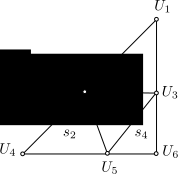
\includegraphics[scale=1.0]{disc_domain}
	\caption{A sample 2D domain discretized with four triangular elements of the first order.}
	\label{fig:disc_domain}
\end{figure}


Two types of meshes are commonly used which are referred to structured meshes and unstructured meshes.
The vertices in a structured mesh lie on grid lines that pass uninterrupted throughout the domain.
As a result, locality information, such as neighboring vertices or edges, can be directly computed from the nodes' indices.
This offers a critical advantage in reducing the overall CPU's memory communication overhead.
However, structured meshes do not adapt well to arbitrary geometries.
Unstructured meshes, on the other hand, place vertices on arbitrary locations in the domain.
As a result, the CPU will require more memory communication overhead in order to process an unstructured mesh.
The key advantage of unstructured meshes though, is that they can better adapt to arbitrary geometries than structured meshes.
In addition, unstructured meshes can allow for increased refinement on local patches situated in interesting domain locations while maintaining coarser patches in other areas.
This results in an improved overall solution accuracy with a lower computational cost.
\figRef{fig:meshTypes} illustrates the two types of meshes.
It is important to note here that, the \gls{acr:fgabp} algorithm does not depend on the type of mesh used; as will later be shown, the \gls{acr:fgabp} was implemented and verified to work with both structured and unstructured meshes.


\begin{figure}
	\centering{
	\subfloat[]{
	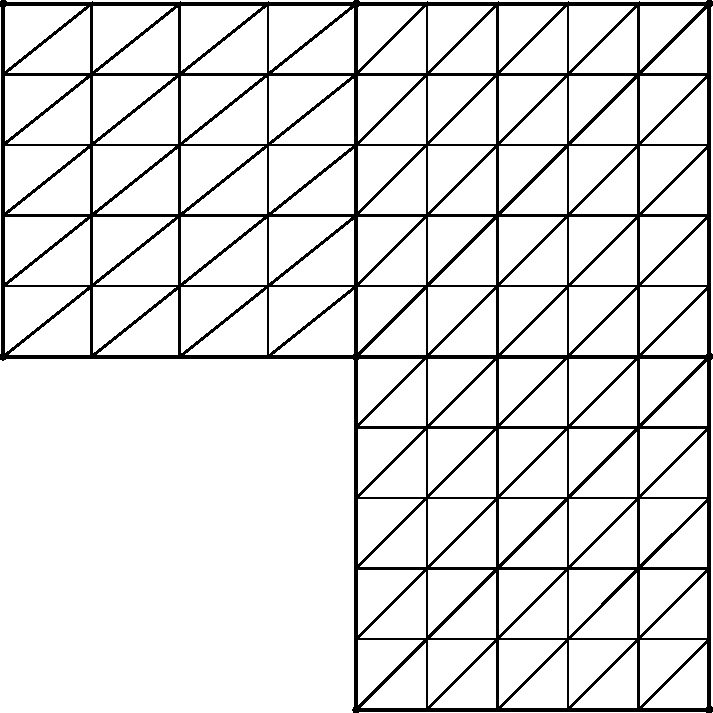
\includegraphics[scale=0.4]{L_shaped_str} \label{fig:strMesh}
	}
  %\hspace{+1mm}
	\subfloat[]{
	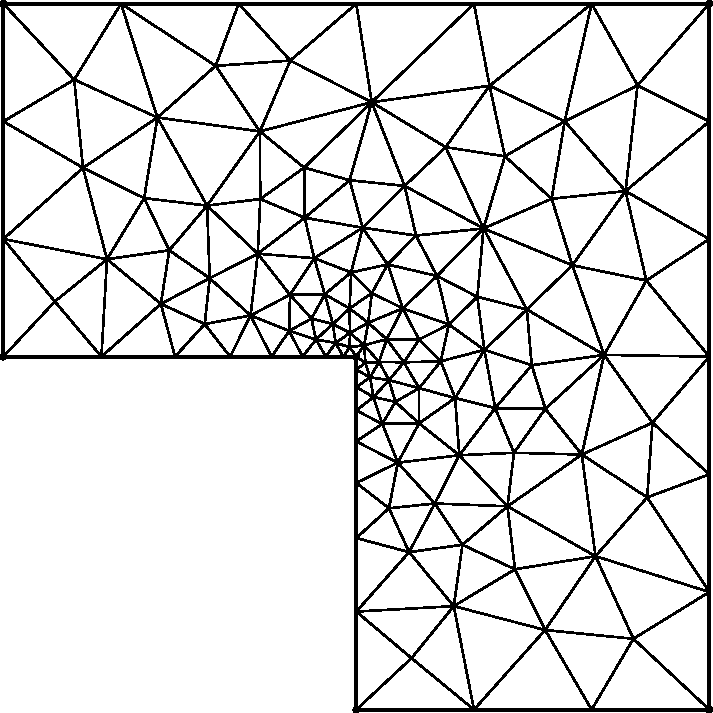
\includegraphics[scale=0.4]{L_shaped_unstr} \label{fig:unstrMesh}
	}
	}
	\caption[Structured and unstructured meshes.]{Structured and unstructured meshes of the L-shaped domain.  \protect\subref*{fig:strMesh} The structured mesh.  \protect\subref*{fig:unstrMesh}~The unstructured mesh. The unstructured mesh provides more refinement at areas of more interest in the domain such as the reentrant corner of the L-shaped region.}
	\label{fig:meshTypes}
\end{figure}

The second step in the \gls{acr:fem} process involves choosing the interpolation polynomials, or as alternatively known the basis functions, in order to approximate the unknown field $U$ within each of the finite elements.
The interpolation polynomials approximate the unknown field using a discrete set of real-valued parameters spatially positioned along each of the finite elements' vertices or edges.
The number of used parameters identify the polynomial interpolation order; for example, a linear triangular element has three parameters positioned along its vertices whereas a second order triangular element has six parameters positioned along its vertices and edges.
For certain \gls{acr:fem} applications, the quality of the approximation will improve with increasing interpolation order; however, the computational complexity of the \gls{acr:fem} will substantially increase.
An expression of this approximation can generally be stated as follows:
\begin{equation}
	U^s(x,y,z) = \sum_{k=1}^{n} U^s_k P^s_k(x,y,z), \,\,\, \forall s \in \mathcal{S}
	\label{eqn:intrPoly}
\end{equation}
where $s$ is the finite element and $\mathcal{S}$ is the total elements' set spanning the domain $\Omega$; $n$ is the number of local discrete values; and $P$ is the interpolating function.
Note that the subscript $k$ in $U^s_k$ refers to the local element node numbering and not the global node numbering; for example, the element $s_3$ in \figRef{fig:disc_domain} has the globally numbered discrete parameters $U_2$, $U_3$ and $U_5$ of globally unique indices $2$, $3$, and $5$.
Typically in \gls{acr:fem} implementations, a mapping of local to global node numbering needs to be defined.
Another important aspect of interpolation polynomials is that the gradient of the field within each element can also be approximated as:
\begin{equation}
	\nabla U^s(x,y,z) = \sum_{k=1}^{n} U^s_k \nabla P^s_k(x,y,z), \,\,\, \forall s \in \mathcal{S}.
	\label{eqn:intrPolyGrad}
\end{equation}
The specifics of the interpolation functions vary for each \gls{acr:fem} scheme; however, they need to maintain the important property of ensuring the continuity of the $U$ field across the finite element edges.


Since the functional $\mathcal{F}$ in \eqnRef{eqn:globalFunc} can, up to a constant, be viewed as an expression of the total energy stored in the system; therefore, $\mathcal{F}$ can be expressed using the sum of energies of each finite element as follows:
\begin{equation}
	\mathcal{F}(U)=\sum_{s\in\mathcal{S}}\mathcal{F}_{s}(U_{s})
	\label{eqn:discFunc}
\end{equation}
where $\mathcal{S}$ is the total elements' set spanning the domain $\Omega$; $U_s$ is the set of the field discrete unknowns, or degrees of freedom, for the finite element $s$; and $\mathcal{F}_s$ is the energy contribution of $s$.
Therefore by rendering stationary the functional in \eqnRef{eqn:discFunc}, an approximate solution to the Helmholtz equation can be found using the \gls{acr:fem} scheme.
Substituting each of \eqnRef{eqn:intrPoly} and \eqnRef{eqn:intrPolyGrad} into \eqnRef{eqn:globalFunc} and applying a standard derivation process, an expression for the local finite element $\mathcal{F}_s$ can, generally, be formulated as:
\begin{equation}
	\mathcal{F}_s(U_s)=\frac{1}{2} U^T_s M_s U_s -B_s^T U
	\label{eqn:elemtFunc}
\end{equation}
in which we refer to $M_s$ as the element characteristic matrix with dimensions $n$-by-$n$ where $n$ is the number of unknowns per element; and $B_s$ is the element source vector.
It is clear that (\ref{eqn:elemtFunc}) can also incorporate the essential boundary conditions as stated for the \gls{acr:bvp}
when $\mathcal{F}_s$ represents a boundary finite element.


Finally, the \gls{acr:fem} solution is computed by executing three main procedures.
First, all the contributions from all the finite elements in terms of the $M_s$ and the $B_s$ elements are added up into a global and sparse linear system of equations. This process is referred to as the assembly process.
Second, the essential boundary conditions are incorporated into the linear system.
Last, the resulting linear system of the form \eqnRef{eqn:aub} is solved using sparse linear solvers such as the \gls{acr:pcg} method.


\subsection{The FEM Parallel Acceleration Issues}

Conventional \gls{acr:fem} implementations consist of two computationally expensive stages which are the sparse matrix $A$ assembly stage, and the solving stage of the linear system using iterative solvers.
Acceleration of these stages using parallel processing will be limited by memory bandwidth issues due to their dependency on the global sparse data-structure of the matrix $A$.
This scalability issue has been the focus of extensive research lately, because computing manufacturers are increasing their chip's computational throughput by adding more cores rather than frequency scaling due to power limitations at the chip level.
Therefore, in order to obtain good performance from emerging parallel computing architectures, the \gls{acr:fem} computation must scale well with parallel computing.
To better illustrate this issue, we consider the \gls{acr:pcg} method, which is a widely used iterative solver for \gls{acr:fem} applications.
The \gls{acr:pcg} solver requires the execution of a number of global algebraic operations in each iteration such as a \gls{acr:smvm} and a preconditioner solve.
The \gls{acr:smvm} operation, in particular, can strongly impact the overall performance of the \gls{acr:pcg} solver since the memory access time will dominate the computational time due the underlying sparse data-structure.
Considering the \gls{acr:smvm} defined as $y=Ax$, where $A$ is a symmetric sparse matrix while $x$ and $y$ are dense vectors, the operation, in its simplest implementations, can be executed as a number of concurrent vector dot products where each dot product consists of $x$ and a row from $A$.
The result from each dot product updates a single value in the output vector $y$.
The dot products are independent of each other, hence they can be executed in parallel.
While this \gls{acr:smvm} approach seems very intuitive and convenient to implement, it actually results in a very poor performance for key reasons.
The data within each row of $A$ is very sparse and require irregular memory access resulting in very low cache hit rates, which substantially increases the CPU's idle time by waiting for data to arrive, causing the CPU to attain only a small fraction of its peak performance.
Without improving the \gls{acr:smvm} execution on a single CPU, parallelizing the \gls{acr:smvm} will not sustain the potential speedup of the parallel platform.
In fact, this issue is even more pronounced for multicore architectures.
As the number of cores increases, the memory requests consequently increases causing a greater bottleneck for the limited memory bandwidth resources.
This in turn severely limits the parallel scalability of the \gls{acr:smvm} operations as will later be demonstrated in the numerical results of \secRef{sec:FMGaBP_res}.


Many attempts are made to improve the performance of the \gls{acr:smvm}; however, typical implementations of the \gls{acr:smvm} yield poor performance of no more than 10-20\% of the peak CPU throughput \cite{bib:Demmel2007OODMVMOEMP}.
Improving the performance of the \gls{acr:smvm} kernel will require sophisticated programming techniques, code transformations, and data-structures that are tailored to specific CPU, cache and memory architectures \cite{bib:DemmelOSKI}.
Specialized sparse data-structures are devised in order to either exploit the sparsity structure of matrices resulting from specific application areas, or target specific \gls{acr:hpc} architectures.
For example, a recent work in \cite{bib:david2010mabpmt} uses blocking schemes to obtain better performance on multicore architectures.
The work in \cite{bib:elkurdi2007hafem,bib:El-Kurdi2008FAAIOSMMFTFEM} uses stripe-based sparse data-structures to accelerate the \gls{acr:smvm} on \glspl{acr:fpga} using a highly parallel hardware architecture based on a systolic pipeline of processing elements.
The numerical results of these efforts indicate that sustaining good performance for all sparse matrices, even within the same \gls{acr:fem} application area, is nearly impossible.
While there also exist generic and optimized libraries such as Trilinos \cite{bib:Trilinos} and PETSc \cite{bib:PETSc}, which can be used to solve the sparse linear system in parallel, obtaining a sustained performance can prove difficult due to the varying sparsity structure of $A$ resulting from different application areas.
In addition, such libraries do not help with the assembly stage of the \gls{acr:fem}, which in many cases can require more time than the solve stage, such as the case for non-linear applications.
In certain cases, matrix reordering can improve the performance of \gls{acr:smvm} by rearranging its elements so that they are more clustered around the main diagonal.
One of the most popular reordering algorithms to improve the \gls{acr:smvm} performance is the \gls{acr:rcm} algorithm \cite{bib:Cuthill1969RTBOSSM}. 
However, reordering requires considerable overhead processing for large matrices.


Another important sparse operation is the sparse matrix assembly and the buildup of the sparse data-structure based on the matrix specific sparsity pattern.
For specialized data-structures, this operation can be very costly.
Parallelizing the matrix assembly also requires special care.
Since the sparse matrix is a shared data-structure, updating the data-structure from different parallel processes needs to avoid memory collisions when accessing shared elements in the matrix.
One way to overcome this issue is by using element coloring schemes, where adjacent elements are given different colors.
Elements of the same color group can then be assembled concurrently.
While, for certain cases, the assembly needs to be done only once and, therefore, its cost can be tolerated; however, for many cases such as \gls{acr:amg} solvers, adaptive refinement, and non-linear applications, the assembly stage can dominate the solve stage.
This is specially so for non-linear applications requiring non-linear solvers, such as the Newton-Raphson method, where the assembly stage must be repeated each linearizing iteration.
Our numerical results in \secRef{sec:FMGaBP_res} demonstrate that the assembly time was considerably long in comparison with the solve time.

As mentioned earlier, computing manufacturers are increasing the number of CPU cores on a single chip as opposed to frequency scaling in order to keep up with Moore's law \cite{bib:moore1965} of increasing chip transistor density; therefore, new and inherently parallel algorithms need to be devised for the \gls{acr:fem} in order to efficiently scale with these parallel computing trends.
In this work, we take a different approach for \gls{acr:fem} computation by directly minimizing the energy functional (\ref{eqn:discFunc}) using a newly derived \gls{acr:fgabp} algorithm.
The \gls{acr:fgabp} algorithm is based on computational inference on \glspl{acr:gm} that exploits the inherent structure of the \gls{acr:fem} problem resulting in localized computation involving dense matrices of very small sizes.
The overall convergence of the algorithm progresses by passing update messages between processing nodes in a flexible manner allowing adaptable memory bandwidth utilization for various \gls{acr:hpc} platforms.
The \gls{acr:fgabp} eliminates the need to generate any large sparse matrices, or use any form of sparse data-structures, by eliminating all the global algebraic operations, including \glspl{acr:smvm}, proving great potential for scalable parallel computational throughput.
Not only the new algorithm efficiently parallelizes the solving stage, but also it allows for an embarrassingly parallel implementation of the assembly stage using only dense and contiguous data-structures.


\section{Graphical Models}


In this section we introduce an overview of the \gls{acr:gm} concept, which is central in the development of the \gls{acr:fgabp} algorithm in \chpRef{chp:FGaBP}.
A \gls{acr:gm} is a graphical representation of a multivariate probability distribution describing a particular problem \cite{bib:PGMkoller2009}.
The \gls{acr:gm} captures the interactions of the random variables which represent the connectivity structure of the underlying problem.
Specifically, the \gls{acr:gm} can assist in the analysis of such problems that require the computation of local parameters about the problem's latent random variables such as the means of the latent random variables or even the joint mean of a subset of latent random variables.
For that purpose, \glspl{acr:gm} can greatly assist in devising inference algorithms that can reuse intermediate results, or exhibit distributed computations that are potentially efficient for parallelism.
For example, executing an inference algorithm such as the \gls{acr:bp} algorithm, described in more details in \secRef{sec:bp}, on a tree structure \gls{acr:gm} can result in optimal execution where only a single computational step is performed per variable regardless of the tree size.
However, practical problems result in more complicated \glspl{acr:gm} than simple trees, where such models can contain loops or clique substructures.
Inference on such \glspl{acr:gm} can take an approximate form with larger number of iterations than loop-free \glspl{acr:gm}.
The number of iterations on loopy \glspl{acr:gm} is typically proportional to the number of variables in the model.  


A \gls{acr:gm} is composed of a set of vertices (or nodes) $\mathcal{V}$ connected by a set of edges $\mathcal{E}$, which is denoted as $\mathcal{G}(\mathcal{V},\mathcal{E})$.
The vertices are denoted by indices such that $\mathcal{V}=\{v_1,v_2,\cdots,v_n\}$.
The edges are links between pairs of vertices and are denoted as follows: given a set of pairs $\mathcal{E} = \{e_{ij} = (v_i,v_j)\, \mid v_i,v_j \in \mathcal{V}\}$ such that $\mathcal{E}\subset \mathcal{V} \times \mathcal{V}$, where $\times$ is the Cartesian product.
\glspl{acr:gm} can either be undirected or directed.
In undirected \glspl{acr:gm} we have the condition: $\text{if } e_{i,j} \in \mathcal{E} \text{ then } e_{j,i} \in \mathcal{E} \, \forall v_i,v_j \in \mathcal{V}$; while, such a condition is not necessarily true for directed \glspl{acr:gm}.
The term undirected edge refers to the fact that diagrammatically, the edges $e_{i,j}$ and $e_{j,i}$ are represented using a single edge without an arrow indicating any particular direction.
\figRef{fig:gmExamples} illustrates examples of directed and undirected \glspl{acr:gm}.
In this work, we only utilize undirected \glspl{acr:gm} for all our developments of parallel algorithms.


\begin{figure}
  \centering
  {
  \subfloat[]{%
  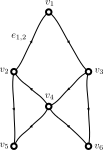
\includegraphics[scale=1.3]{directed_gm} \label{fig:dgm}
  }
  \hspace{1cm}
  \subfloat[]{%
  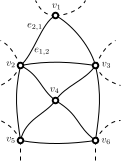
\includegraphics[scale=1.3]{undirected_gm} \label{fig:ugm}
  }
  }
  \caption[Examples of directed and undirected \acrshortpl{acr:gm}.]{Examples of directed and undirected \glspl{acr:gm}. \protect\subref*{fig:dgm}~Loop free directed \gls{acr:gm}. \protect\subref*{fig:ugm}~Loopy undirected \gls{acr:gm}.}
  \label{fig:gmExamples}
\end{figure}


Using a \gls{acr:gm} of a particular distribution, an inference algorithm can be devised based on the interactions between the latent variables in the model as well as the information propagating along its edges, therefore the following additional notations are required in order to simplify the formulation.
A random variable $U$ located on a vertex $v_i$ is denoted as $U_i$.
A message $m$ sent on an edge $e_{i,j}$ from vertex $i$ to vertex $j$ is denoted as $m_{ij}$.
It is worth noting that in undirected \glspl{acr:gm} where the edges $e_{i,j}$ and $e_{j,i}$ coexist, it is not necessarily true that the messages $m_{ij}$ and $m_{ji}$ are equal.

In essence, the messages in a \gls{acr:gm} describe a probability distribution in terms of either the target node variable $m_{ij}(U_j)$ or the source node variable $\eta_{ij}(U_i)$ which actually constitutes the flow of information in the \gls{acr:gm}.
Sometimes, we are interested in the joint distribution of a subset of random variables; if no confusion can arise, a subset of variables can simply be denoted as follows: if $c=\{1,2,\cdots,n\}$ then $U_c=\{U_1,U_2,\cdots,U_n\}$.
Similarly, a subset of vertices is denoted as $v_c=\{v_1,\cdots,v_n\}$.
The number of individual variables in $U_c$ is referred to as the cardinality of $U_c$ and is denoted by $\cardinal{U_c}$.


A clique $C(v_c)$ in a graph $\mathcal{G}(\mathcal{V},\mathcal{E})$ is a subset of nodes $v_c$ that are fully connected such that if $v_i,v_j \in v_c$, then $e_{i,j} \in \mathcal{E}$.
A clique is maximal if, and only if, there is no other node from outside the clique that can be added to it and still form a clique.
In other words, only a nonmaximal clique is a proper subset of a maximal clique.
The simplest example of a clique is a clique formed by any pair of nodes connected by an edge.
Also, any three nodes connected by three undirected edges form a clique. 


Undirected \glspl{acr:gm} represent a class of distributions that can be factorized based on cliques in the graph.
Let $\mathcal{C}$ be the set of maximal cliques in an undirected \gls{acr:gm},  then a family of distributions can be defined as follows:
\begin{equation}
	\mathcal{P}(U) = \frac{1}{Z} \prod_{C \in \mathcal{C}} \Psi_C(U_c) \label{eqn:maxcliqP}
\end{equation}
where $Z$ is a normalizing constant and $\Psi_c(U_c)$ is usually referred to as a compatibility function which also can be regarded as a local distribution of the clique variables $U_c$.
Such families of \glspl{acr:gm} are referred to as \gls{acr:mrf} or Gibbs distributions \cite{bib:Wainwright2008GMEFAVI}.
The maximal cliques requirement for \eqnRef{eqn:maxcliqP} can sometimes be relaxed to nonmaximal cliques.
For example, consider the following factorized distribution:
\begin{equation}
	\mathcal{P}(U) = \frac{1}{Z} \prod_{(i,j) \in E} \Psi_{i,j}(U_i,U_j) \prod_{i \in V} \Phi_i(U_i) \label{eqn:pwcliqP}
\end{equation}
where $\Psi_{i,j}(U_i,U_j)$ is referred to as the pairwise compatibility function and $\Phi_i(U_i)$ is the self potential function.
Distributions of this form can be represented by a \gls{acr:gm} that is pairwise connected, which we refer to as \gls{acr:pwgm}, where each vertex represents a variable node.


Since, in general, distributions corresponding to loopy undirected \glspl{acr:gm} contain factors that have coupled, or correlated, variable sets, inference on such models is not necessarily a trivial task.
However, the factorization structure of these distributions, as exposed by the \gls{acr:gm}, can be exploited by certain inference algorithms to produce computationally efficient algorithms. 


Distributions of the form \eqnRef{eqn:maxcliqP} are more conveniently represented using a special type of graph referred to as a \gls{acr:fg} \cite{bib:Kschischang2001FGATSA}.
\glspl{acr:fg} are bipartite graphs denoted as $\mathcal{G}(\mathcal{V},\mathcal{F},\mathcal{E})$, where there are two types of vertices, the vertex $v_i \in \mathcal{V}$ representing the variable nodes and the vertex $f_a \in \mathcal{F}$ representing the compatibility (or factor) functions $\Psi_a(U_a)$.
An edge $e_{i,a}$ in a \gls{acr:fg} connects a vertex $v_i \in \mathcal{V}$ to a vertex $f_a \in \mathcal{F}$ only when the corresponding vertex variable $U_i$ is an argument of the factor function $\Psi_a(U_a)$.
\figRef{fig:pw_vs_fg} shows a \gls{acr:pwgm} model and the corresponding \gls{acr:fg} with factor functions based on maximal cliques.
\glspl{acr:fg} are particularly useful when nonmaximal cliques are also configured; in such a case, different message update algorithms can be devised for the same problem resulting in different implementations with different numerical properties.
This feature will be exploited by our \gls{acr:fg} model for the \gls{acr:fem} problem, the \acrshort{acr:femfg} model, later introduced in \chpRef{chp:FGaBP}.
The \gls{acr:femfg} model can be used to produce variants of the \gls{acr:fgabp} algorithm, later described in \secRef{sec:elmMerg}, which has higher memory communication efficiency.  


\begin{figure}
	\centering
	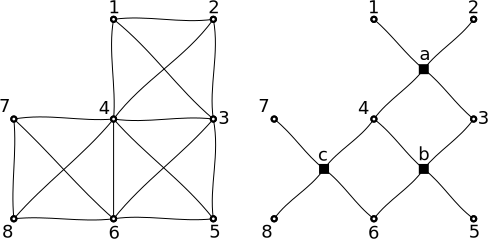
\includegraphics[scale=.9]{pw_vs_fg}
	\caption[The \acrshort{acr:pwgm} and the \acrshort{acr:fg} model.]{The \gls{acr:pwgm} (or \gls{acr:mrf}) on the left and the corresponding \gls{acr:fg} model configured with maximal cliques on the right, variable nodes are represented by circles and factor nodes are represented by squares.}
	\label{fig:pw_vs_fg}
\end{figure}


For general \glspl{acr:gm}, we will denote the number of variable nodes or vertices as \gls{acr:nv}, the number of edges as \gls{acr:ne} and the number of factor nodes, when present, as \gls{acr:nf}.
In addition, we will typically use small letters such as $n$ and $n_e$ to denote the local factor or clique quantities such as the number of vertices and edges correspondingly.



\section{The Belief Propagation Algorithm}
\label{sec:bp}


The \glsfirst{acr:bp} algorithm, as proposed by Pearl in \cite{bib:Pearl88ProbabilisticReasoning}, is a message passing algorithm on \gls{acr:gm} that efficiently computes the marginal distribution of each variable node by recursively sharing intermediate results.
If the \gls{acr:gm} is a tree, then \gls{acr:bp} is guaranteed to converge to exact marginals.
However, if the \gls{acr:gm} contains cycles, as typically the case in many practical applications, then \gls{acr:bp} takes an iterative form, referred to as \glsfirst{acr:lbp}, which can be used to obtain an approximation for the marginals \cite{bib:Pearl88ProbabilisticReasoning,bib:Yedidia2004CFEAAGBPA,bib:Weiss01CorrectnessBelief,bib:Wainwright03tbrfasp}.
\Gls{acr:bp} recently showed excellent empirical results in certain applications, such as machine learning, expert systems, computer vision, and channel decoding \cite{bib:Kschischang2001FGATSA, bib:Wainwright2008GMEFAVI,bib:Luby2001ILDPC,bib:Mceliece98turbodecoding,Richardson2001CLDPC,bib:cv1999,bibSun2003SMU,bib:Frey2001NIPS,bib:Kolmogorov2006ctr,bib:Weiss2005gobp,bib:Szeliski2008CS}.


\subsection{Belief Propagation on Factor Graph Models}


Executing \gls{acr:bp} on \glspl{acr:fg} consists of passing two types of messages.
A factor node message $m_{ai}$ sent from a factor node $\Psi_a$ to a connected variable node $U_i$; and a variable node message $\eta_{ia}$ sent back from the variable node $U_i$ to the factor node $\Psi_a$.
\Gls{acr:bp} messages on \gls{acr:fg} models are probability distributions; such that, the factor node message $m_{ai}$ constitutes a distribution in terms of the continuous random variable $U_i$, or the most probable state of $U_i$, as observed from the factor node $f_a$ with local function $\Psi_a$.
In return, the variable node message $\eta_{ia}$ constitutes a distribution in terms of $U_i$ by combining messages from all connected factor nodes excluding the message from the factor $f_a$.
The general \gls{acr:bp} update rules on \glspl{acr:fg} are formulated as follows:
\begin{align}
	m_{ai}^{(t)}(U_{i}) & \propto \underset{U_{\mathcal{N}(a)\setminus i}}{\int}\Psi_{a}(U_{a})\prod_{j\in\mathcal{N}(a)\setminus i}\eta_{ja}^{(t_\star)}(U_{j})\ \mathrm{d} U_{\mathcal{N}(a)\setminus i} \label{eqn:genFNUM}\\
	\eta_{ia}^{(t)}(U_{i}) & \propto \prod_{k\in\mathcal{N}(i)\setminus a}m_{ki}^{(t_\star)}(U_{i}) \label{eqn:genVNUM}\\
	b_{i}^{(t)}(U_{i}) & \propto \prod_{k\in\mathcal{N}(i)}m_{ki}^{(t)}(U_{i}) \label{eqn:genB}
\end{align}
where $t$ and $t_\star$ are iteration counts such that $t_\star \leq t$; \neih{a} is the set of all node indices connected to node $a$, referred to as the neighborhood set of node $a$; \neihMinus{a}{i} is the neighborhood set of $a$ minus node $i$ index; $b_i(U_i)$ is referred to as the belief at node $i$.  
The integral in \eqnRef{eqn:genFNUM} is a multidimensional integral of the random variable set $U_{\mathcal{N}(a)\setminus i}$ each integrated over all of their possible values.


It is important to note that message updates are performed according to a particular schedule.
For example, if we would use a fully parallel schedule, that is $t = t - 1$, then all factor and variable nodes will update their messages simultaneously based on the message values of the previous iteration; this update schedule is also referred to as synchronous update.
Alternatively we could traverse each variable or factor node sequentially based on a particular order, and then compute new messages based on the most recently available messages; this update schedule is also referred to as asynchronous updates.
Such a schedule does not offer the most potential for parallelism, but it was found empirically to exhibit the fastest to converge rate \cite{bib:Elidan06ResidualBP}.

\subsection{Belief Propagation on Pairwise Graphical Models}
\label{sec:pwgabp}


Considering \glspl{acr:pwgm} resulting from distributions with pairwise compatibility functions as shown in \eqnRef{eqn:pwcliqP}, each node sends and receives messages along all the pairwise edges connected to it.
Since variable nodes only communicate with other variable nodes of the same type, there can be only one type of message computed along the pairwise edges.
The general \gls{acr:bp} update rule for \glspl{acr:pwgm} is stated as follows:
\begin{equation}
	m_{ij}^{(t)}(U_j) \propto \underset{U_i}{\int}\Psi_{ij}(U_i,U_j)\Phi_i(U_i)\prod_{k\in\mathcal{N}(i)\setminus j}m_{ki}^{(t_\star)}(U_i)\mathrm{d} U_i. \label{eqn:genBPpw}
\end{equation}
The integral in \eqnRef{eqn:genBPpw} is taken for the single random variable $U_i$ over all its possible values.
A message $m_{ij}(U_j)$ is communicated from variable node $v_i$ to variable node $v_j$ over the edge $e_{i,j}$ using messages previously received from the neighborhood $\mathcal{N}(i)\setminus j$.
Once the messages converge, the marginal distribution for each variable can be obtained as:
\begin{equation}
	b_{i}^{(t)}(U_i) \propto \Phi_i(U_i) \prod_{k\in\mathcal{N}(i)}m_{ki}^{(t)}(U_i). \label{eqn:genBBPpw}
\end{equation}


\subsection{The Gaussian Belief Propagation Solver on Pairwise Graphical Models}


In this section we present a brief overview of the \glsfirst{acr:pwgabp} \cite{bib:Shental2008GBPSSLE,bib:Weiss01CorrectnessBelief} which was a recently introduced as a solver for linear systems of equations based on \gls{acr:bp} executed on \gls{acr:pwgm}.
While our initial experimentations with \gls{acr:pwgabp} for linear systems resulting from \gls{acr:fem} applications reveal that its performance does not match the existing state-of-the-art solvers such as \gls{acr:icpcg} and multigrid based solvers for large systems; it does offer however an important insight on the potential of using \gls{acr:bp} style algorithms to parallelize the \gls{acr:fem} problem as discussed in Chapters \ref{chp:PW-GaBP} and \ref{chp:relGaBP}.
In addition, the \gls{acr:pwgabp} requires the assembly of the large sparse linear system as in \eqnRef{eqn:aub} or the sparse matrix $A$, which is a costly step in the FEM process.


A Gaussian \gls{acr:pwgm} model is formulated by taking the exponential of the negated quadratic, defined in \eqnRef{eqn:quad}, as:
\begin{equation} 
	\label{eqn:maxGa}
	\mathcal{P}(U) = \frac{1}{Z}\exp(- \frac{1}{2}U^T A U + b^T U + c) 
\end{equation}
where $Z$ is a constant.
It can be shown that the solution of the linear system $u_{\star}=A^{-1}b$ is the maximum point of $\mathcal{P}$ which is also the point where the quadratic \eqnRef{eqn:quad} is minimum.
The exponential expression in (\ref{eqn:maxGa}) is a multivariate Gaussian probability distribution where the Gaussian mean vector $\mu$ equals the solution to the linear system $\mu = A^{-1} b$.
Hence the solution to the linear system can alternatively be obtained by executing the \gls{acr:bp} algorithm on the Gaussian \gls{acr:pwgm} represented by $\mathcal{P}$ in order to obtain its marginal means.

The Gaussian \gls{acr:pwgm} is constructed using the sparse matrix $A$ as follows.
The matrix $A$ can be viewed as an undirected graph where each nonzero element ($A_{ij} \neq 0$) represents an undirected edge between a pair of variable nodes indexed as $v_i$ and $v_j$.
Equivalently, we can factor the graph's distribution $\mathcal{P}$ into nodal functions $ \phi_i(U_i) \triangleq  \exp(- \frac{1}{2} A_{ii}U_i^2 + b_iU_i)$ and edge functions $\psi_{i,j}(U_i,U_j) \triangleq \exp(- \frac{1}{2} U_i A_{ij} U_j) $.
\gls{acr:bp} executing on Gaussian \gls{acr:pwgm} results in messages communicated between variable nodes as follows.
Each node $v_i$ computes a new message towards node $v_j$ on a particular edge $e_{i,j}$  using all messages received from nodes in the neighborhood $\mathcal{N}(i)$ of node $v_i$ excluding the message received from $v_j$.
The message update from each node is performed either sequentially or concurrently subject to a specific schedule.
Since the underlying distribution is Gaussian, the belief updates will be based on propagating only two parameters $\alpha$ and $\beta$, as shown below:
\begin{align}
\label{eqn_GaBPUpdateP}
\alpha_{ij}^{(t)} & = -A_{ij}^2 (\alpha_{i \setminus j}^{(t_\star)})^{-1} \\
\label{eqn_GaBPUpdateM}
\beta_{ij}^{(t)} & = -A_{ij} \beta_{i \setminus j}^{(t_\star)} (\alpha_{i \setminus j}^{(t_\star)})^{-1} \\
\intertext{where:}
\label{eqn_a_i_minus_j_bc}
\alpha_{i \setminus j}^{(t_\star)} & =  \alpha_i^{(t_\star)} - \alpha_{ji}^{(t_\star)} \\
\label{eqn_b_i_minus_j_bc}
\beta_{i \setminus j}^{(t_\star)} & = \beta_i^{(t_\star)} - \beta_{ji}^{(t_\star)} \\
\intertext{and:}
\alpha_i^{(t)} & = A_{ii} + \sum_{k \in N(i)} \alpha_{ki}^{(t)} \\
\beta_i^{(t)} & = b_i + \sum_{k \in N(i)} \beta_{ki}^{(t)} .
\end{align}


For large sparse systems, the overall \gls{acr:pwgabp} computational complexity per iteration is $\bigo{lN}$,  where $N$ is the number of unknowns and $l$ is a constant ($l \ll N$) determined by the sparsity of the underlying problem, for example the average number of links per node.  
The marginal means, constituting the approximate solution, can then be computed by:
\begin{equation}
\label{eqn_x_i}
\bar{U}_i^{(t)} = \frac{\beta_i^{(t)}}{\alpha_i^{(t)}}. 
\end{equation}





GaBP was shown in \cite{bib:Johnson2006WIAGBP} to converge for a particular class of matrices referred to as the walk-summable model.
The walk-summability condition states that the spectral radius of the normalized off-diagonals of $A$ is less than 1 in the absolute sense, that is $\rho(\vert I - D^{-\frac{1}{2}} A D^{-\frac{1}{2}}\vert) < 1$, where $D$ is the diagonal elements of $A$.
Such class of matrices includes the symmetric positive-definite diagonally dominant systems that arise from many \gls{acr:fem} applications.
\gls{acr:pwgabp} is one of the algorithms implemented by the parallel library Graphlab \cite{bib:graphlab2010} aimed primarily at machine learning applications.


\section{Convergence Testing}
\label{sec:convtest}
In practical implementations of the Gaussian \gls{acr:bp} algorithms, the $l^2$-norm of the differences in the successive approximate solutions, the relative norm for short, can be used as a computationally efficient measure to test the convergence of the algorithm.
The relative norm ($e_r$) is computed as follows:
\begin{align} 
	e^{(t)}_r & =  \frac{\parallel \bar{u}^{(t)} - \bar{u}^{(t-1)} \parallel_2}{\parallel \bar{u}^{(t)} \parallel_2} \notag \\
		& = \left(\frac{\sum_{i=1}^{N} (\bar{u}_i^{(t)} - \bar{u}_i^{(t-1)})^2} {\sum_{i=1}^{N} (\bar{u}_i^{(t)})^2}\right)^{\frac{1}{2}} \label{eq_relErr}
\end{align}
where $(t)$ is the iteration number, $\bar{u}^{(t)}$ is the solution vector estimate at iteration $(t)$ and $\bar{u}_i$ is the solution estimate at node $i$.
The algorithm can be terminated when the relative norm reaches a certain tolerance value.
The relative norm is also used for our development of the faster convergent relaxed \gls{acr:pwgabp} algorithm introduced in \chpRef{chp:relGaBP}.

Another measure for convergence is the normalized residual $l^2$-norm, which is computed as follows:
\begin{equation} 
	R^{(t)} = \frac{\parallel b - A\bar{u}^{(t)} \parallel_2}{\parallel b \parallel_2}
\end{equation}
The residual $R$ provides an upper bound for the relative norm; however, the relative norm is used in practice for \gls{acr:pwgabp} to test convergence since it is less costly to compute by avoiding the \gls{acr:smvm} operation ($A\bar{u}^{(t)}$).
However, in \gls{acr:cg} and multigrid algorithms, the residual is typically used for convergence testing since it is iteratively computed as part of these algorithms.
In addition, the residual is used as the final convergence verification criteria in our experiments when we compare different algorithms.

\section{The Condition Number and Diagonal Dominance} 
\label{sec:cndd}
The Condition number of a matrix is defined as:
\begin{equation}
k\left(A\right) \triangleq \frac{\lambda_{max}\left(A\right)}{\lambda_{min}\left(A\right)}
\end{equation} 
where $\lambda_{max}\left(A\right)$ and $\lambda_{min}\left(A\right)$ are the largest and smallest eigenvalues of $A$.
In numerical linear algebra, the condition number measures the sensitivity of the solution of the linear system to small perturbations in $A$.
It may also be used to bound the convergence rate of iterative solvers of linear systems.
Well-conditioned matrices have $k\left(A\right)\approx 1$ while ill-conditioned matrices can have a much larger condition number.

The matrix $A$ is known to be \gls{acr:wdd} if 
\begin{equation}
|a_{ii}| \geq \sum_{j\neq i} |a_{ij}| \quad\text{for all } i, \label{eq:diagDom}
\end{equation}
with strict inequality ($>$) for at least one index $i$.
If the inequality is replaced by ($>$) for all $i$, then the matrix $A$ is referred to as \gls{acr:sdd}.


\section{Speedup}


The execution time speedup (\gls{acr:su}) is the performance measure used in our experiments.
The \gls{acr:su} is defined as the ratio of the execution times of two algorithms or implementations and computed as follows:
\begin{equation}
	\text{SU} = \frac{\text{execution time of algorithm $Y$}}{\text{execution time of algorithm $X$}}
	\label{eqn:suET}
\end{equation}
which states the speedup of algorithm $X$ over algorithm $Y$.
If algorithm $X$ is the parallel implementation of a sequential algorithm $Y$, then this is referred as the parallel \gls{acr:su}.
